% begin module polar-symmetry
\begin{frame}
\frametitle{Symmetry}
\begin{itemize}
\item<1-| alert@2>  If the polar equation is unchanged when $\theta$ is replaced by $-\theta$, the curve is symmetric about the polar axis.
\item<1-| alert@3>  If the equation is unchanged when $\theta$ is replaced by $\pi + \theta$, the curve is symmetric under rotation about the pole.
\item<1-| alert@4>  If the equation is unchanged when $\theta$ is replaced by $\pi - \theta$, the curve is symmetric about the vertical line $\theta = \frac{\pi}{2}$.
\end{itemize}
\begin{center}
\psset{xunit=0.65cm, yunit=0.65cm, algebraic=true}%
\begin{pspicture}(-3.4, -3.4)(3.4,3.4)
\tiny
\psaxes[labels=none, ticks=none, arrows=<->](0,0)(-3.3, -3.3)(3.3, 3.3)%
\uncover<2>{%
\fcDrawPolar[linecolor=red, plotpoints=1000]{0}{6.28319}{2+cos(3*t)}%
\fcAngle[linecolor=\fcColorGraph, arrows=->] {0}{1.047197551}{0.6}{$\theta$}%
\psline[linecolor=blue](0,0)(0.500000, 0.866025)
\fcFullDot{0.500000}{0.866025}%
\rput[bl](0.6, 1){$(\rho, \theta)$}%
\fcAngle[linecolor=\fcColorGraph, arrows=->] {0}{-1.047197551}{0.8}{$-\theta$}%
\psline[linecolor=blue](0,0)(0.500000, -0.866025)
\fcFullDot{0.500000}{-0.866025} %
\rput[tl](0.6, -1){$(\rho, -\theta)$}%
}%
\uncover<3>{%
\fcDrawPolar[linecolor=red, plotpoints=1000] {0}{6.28319}{2+cos(2*t-0.5)}%
\fcAngle[linecolor=\fcColorGraph, arrows=->] {0}{1.047197551}{0.8}{$\theta$}%
\psline[linecolor=blue](0,0)(0.988202, 1.711616)
\fcFullDot{0.988202}{1.711616}%
\rput[b](1, 1.8){$(\rho, \theta)$}%
\fcAngle[linecolor=\fcColorGraph, arrows=->] {0}{4.188790205}{0.6}{$\pi+\theta$}%
\psline[linecolor=blue](0,0)(-0.988202, -1.711616)
\fcFullDot{-0.988202}{-1.711616}%
\rput[t](-1, -1.8){$(-\rho, \theta)$}%
}%
\uncover<4>{%
\fcDrawPolar[linecolor=red, plotpoints=1000]{0}{6.28319}{2+sin(5*t)}%
\fcAngle[linecolor=\fcColorGraph, arrows=->] {0}{0.523598776}{0.8}{$\theta$}%
\psline[linecolor=blue](0,0)(2.165064, 1.250000)
\fcFullDot{2.165064}{1.250000}%
\rput[b](2.1, 1.3){$(\rho, \theta)$}%
\fcAngle[linecolor=\fcColorGraph, arrows=->] {0}{2.617993878}{0.5}{$\pi-\theta$}%
\psline[linecolor=blue](0,0)(-2.165064, 1.250000)
\fcFullDot{-2.165064}{1.250000}%
\rput[b](-2.1, 1.3){$(\rho,\pi- \theta)$}%
}%
\end{pspicture}
%\ \only<handout:1| -2>{%
%\uncover<2>{%
%\ 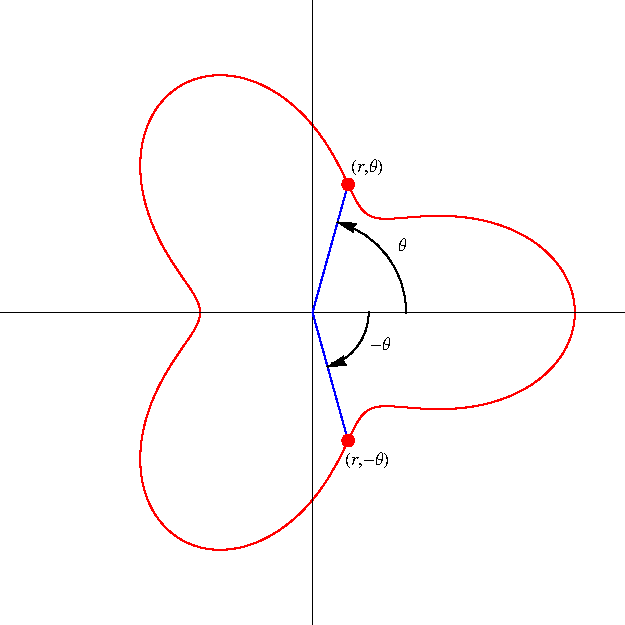
\includegraphics[height=3cm]{polar-curves/pictures/11-03-symmetrya.pdf}%
%}}%
%\only<handout:2| 3>{%
%\ 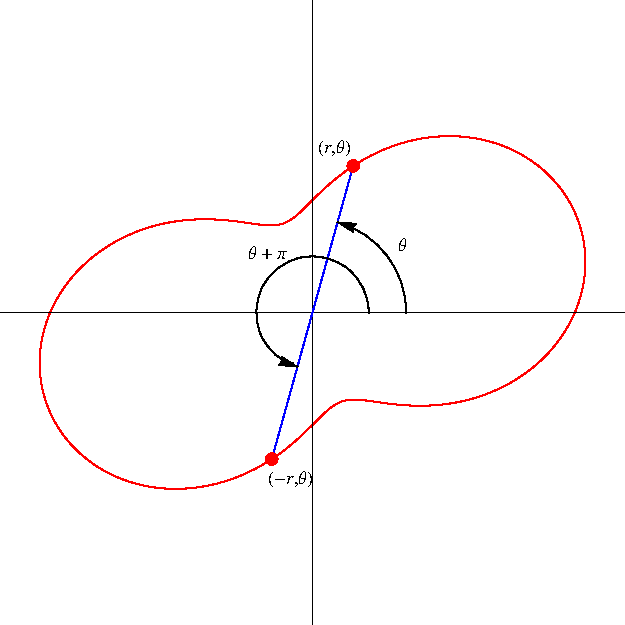
\includegraphics[height=3cm]{polar-curves/pictures/11-03-symmetryb.pdf}%
%}%
%\only<handout:3| 4->{%
%\ 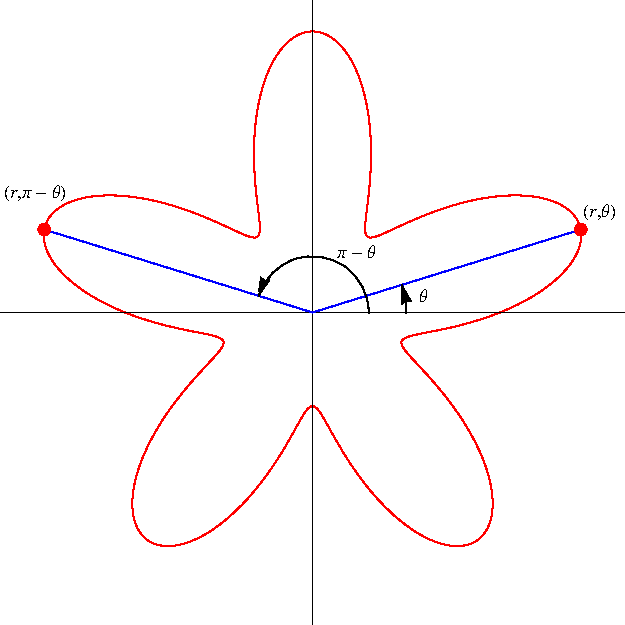
\includegraphics[height=3cm]{polar-curves/pictures/11-03-symmetryc.pdf}%
%}
\end{center}
\end{frame}
% end module polar-symmetry
